\documentclass{beamer}

\usepackage[british]{babel}
\usepackage{graphicx,hyperref,ru,url}

\title[AI@Webscale Presentation]{
  AI at the Webscale Project Results}

\author[Bas Bootsma, Fenno Vermeij]{Bas Bootsma \& Fenno Vermeij}

\institute[Radboud University Nijmegen]{Radboud University Nijmegen}

\date{\today}

\begin{document}

\begin{frame}
  \titlepage
\end{frame}

\begin{frame}
	\frametitle{Approach}	
	\begin{itemize}
		\item Epsilon-greedy
		\item Gibbs-sampling
		\item Thompson-sampling
	\end{itemize}
\end{frame}

\begin{frame}
	\frametitle{Model}
	
		\begin{align*} r = \beta_0 + \beta_{x_1} c_1 + &\ldots + \beta_{x_k} c_k + \\
	    \beta_{y_1} a_1 + &\ldots + \beta_{y_l} a_l + \\
	    \beta_{z_1} c_1a_1 + &\ldots + \beta_{z_m} c_ka_l 
	    \end{align*}
	    \begin{itemize}
		\item Reward for update: use \emph{price} $\cdot$ \emph{effect} instead of \emph{effect}
	\end{itemize}
\end{frame}

\begin{frame}
	\frametitle{Visualization of policy}
	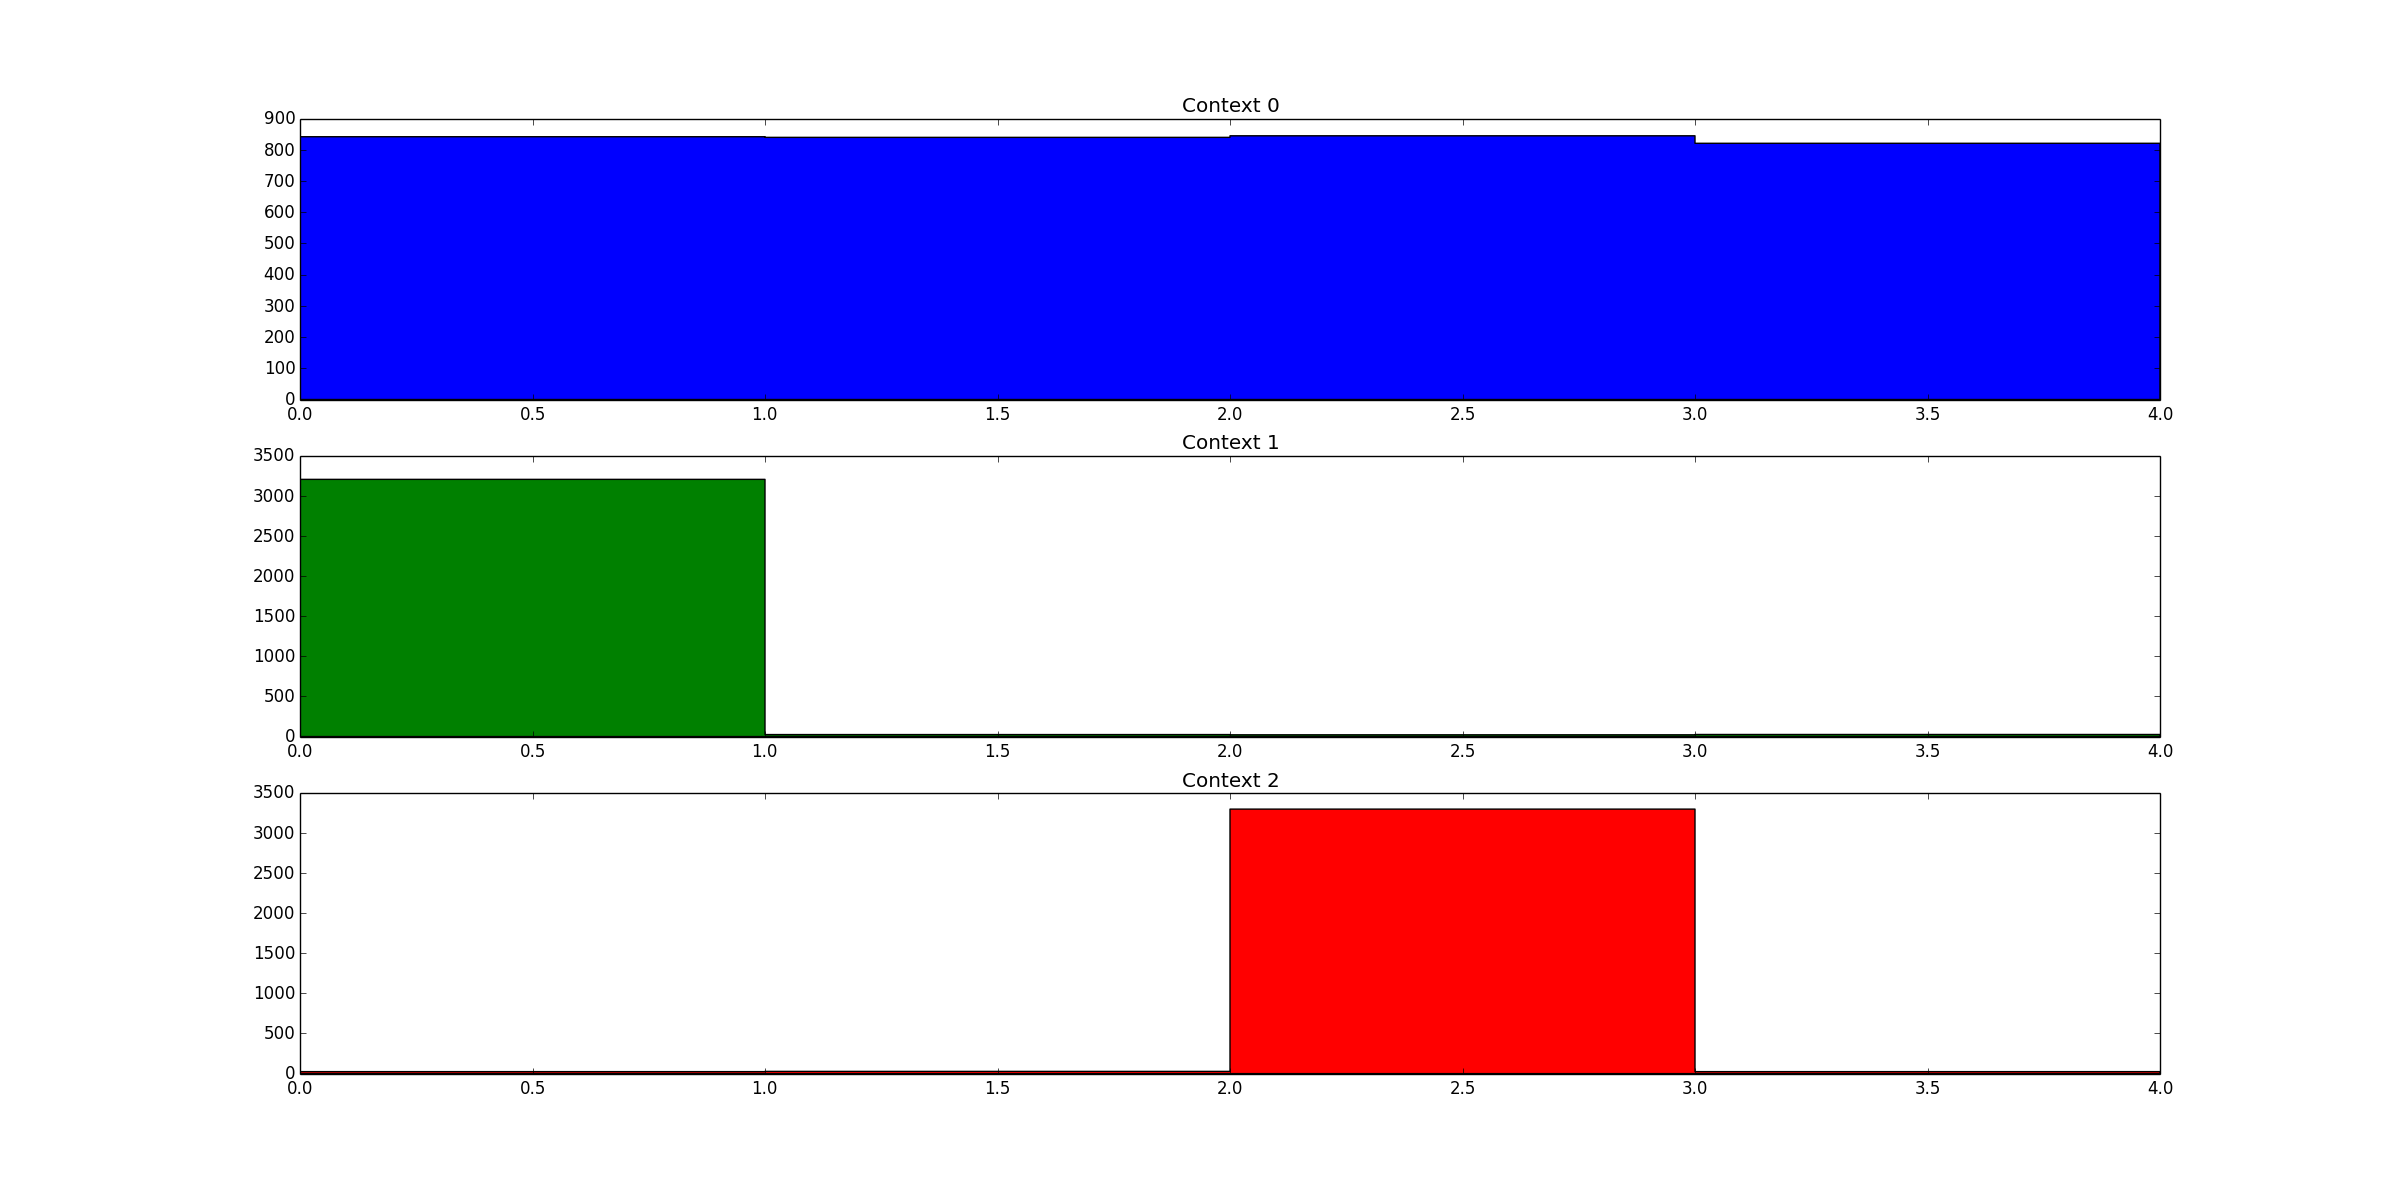
\includegraphics[width=\textwidth]{test.png}
	\begin{itemize}
		\item Pre-defined distribution for $3$ context parameters, and $4$ arms
	\end{itemize}
\end{frame}

\begin{frame}
	\frametitle{Visualization of context vs. proposal}
	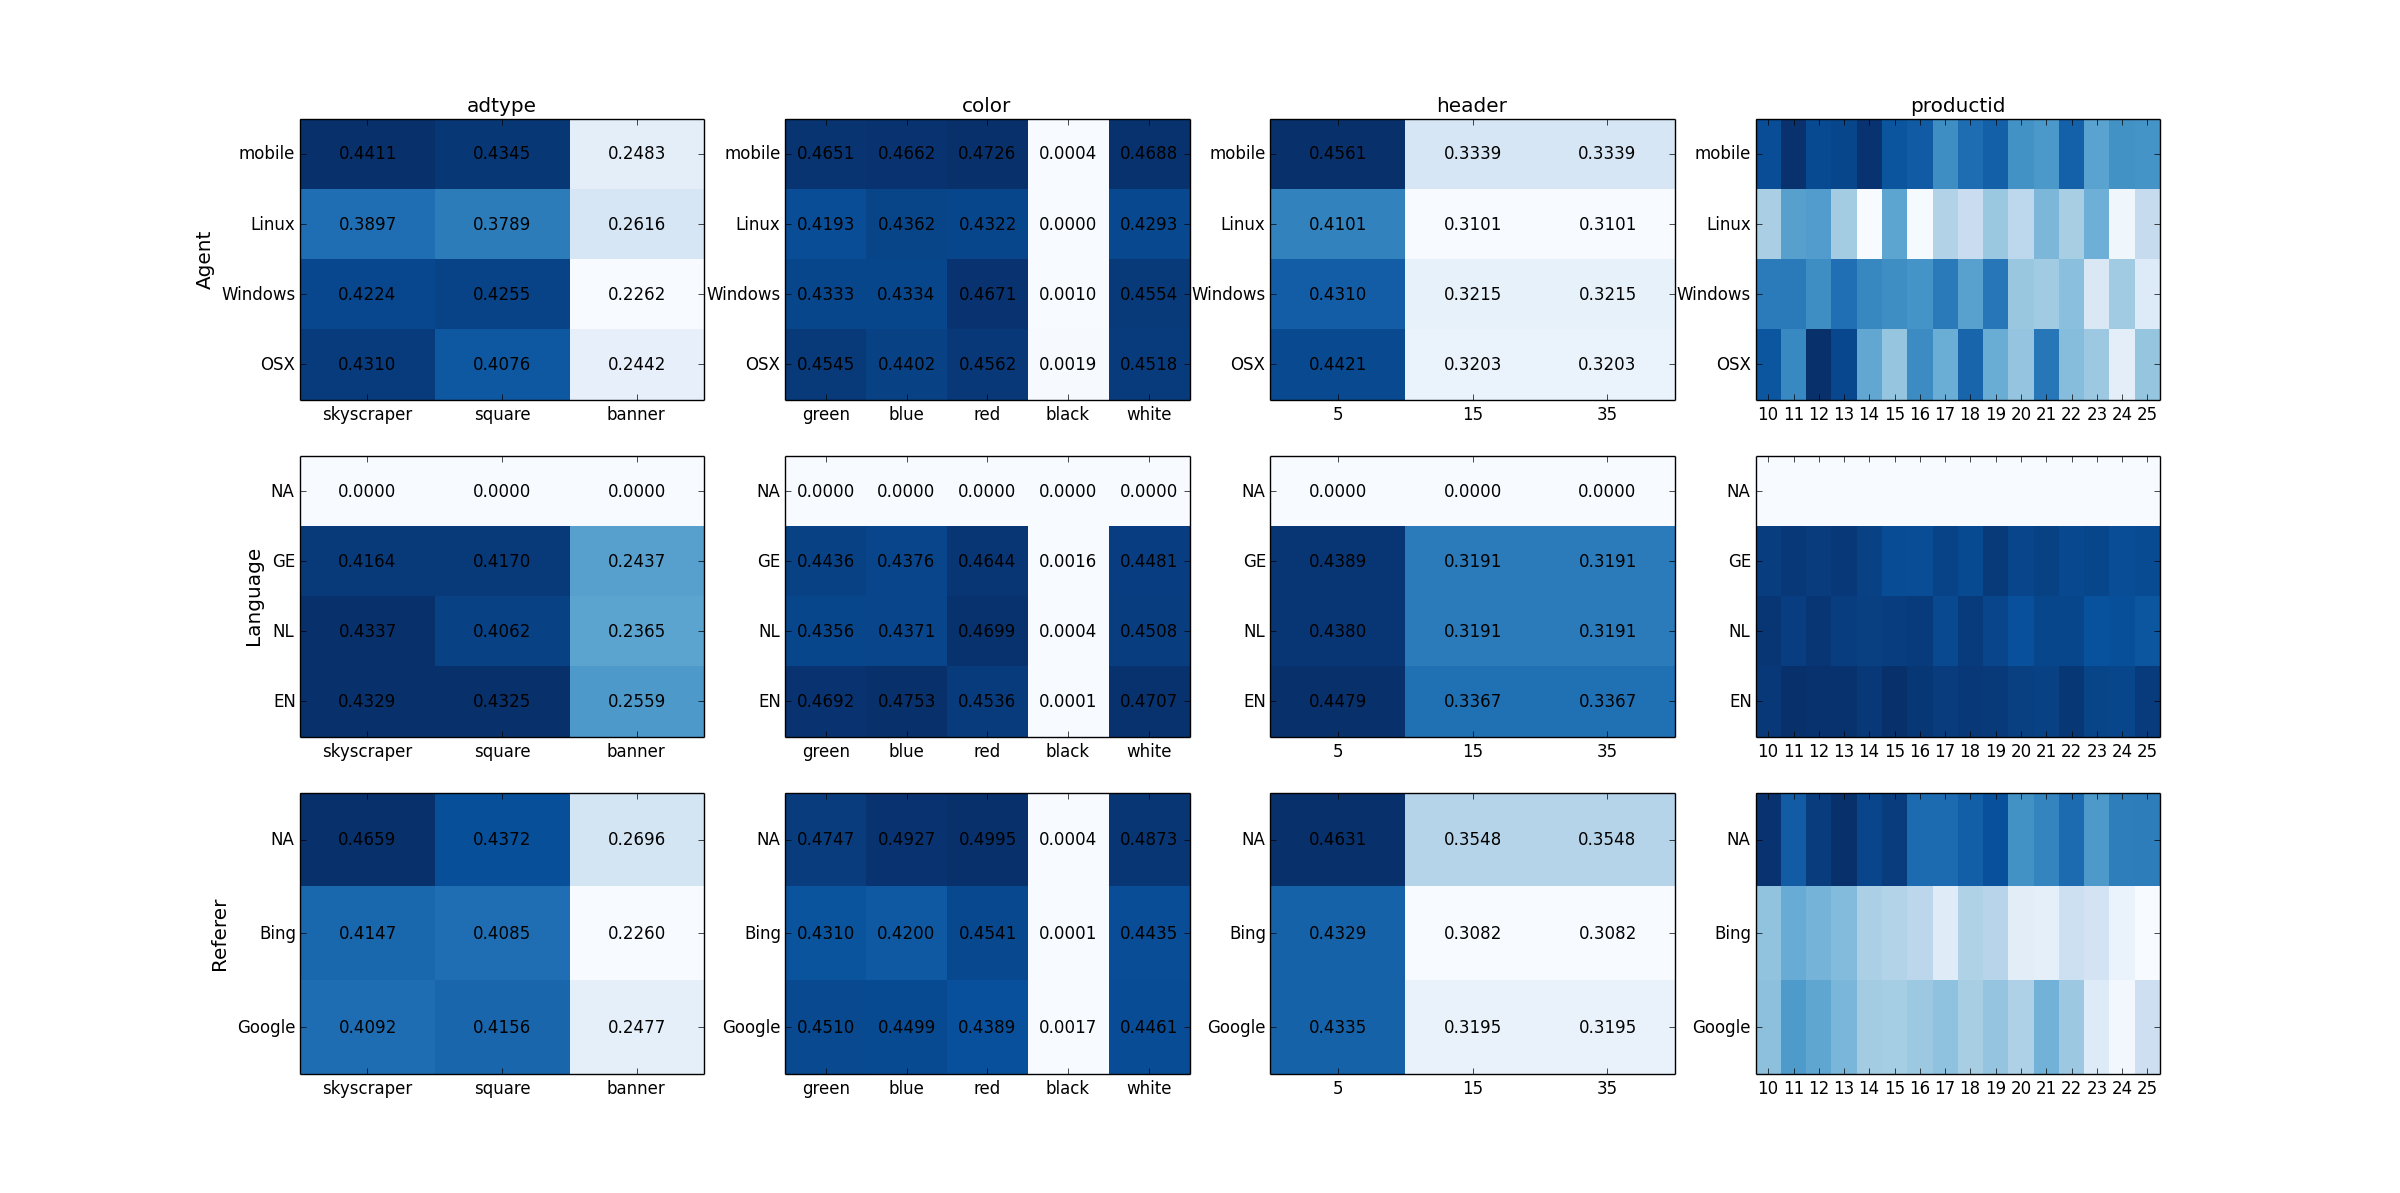
\includegraphics[width=\textwidth]{viewer.png}
	\begin{itemize}
		\item Every possible combination of proposal parameters, except \emph{price} = $1$
	\end{itemize}
\end{frame}


\begin{frame}
	\frametitle{Miscellaneous improvements}
	\setbeamercovered{transparent}
	\begin{itemize}
		\item<1,5| alert@5> Price: Maximize polynomial: $\beta_0 + \beta_1 \cdot p + \beta_2 \cdot p^2$ instead of bucketing: [1, 5, 10, 15, 20, 25, 30, 35, 40, 45, 50]
		%in buckets: [1, 5, 10, 15, 20, 25, 30, 35, 40, 45, 50]
		\item<2,5| alert@5> Multivariate Gaussian speedup: using Cholesky transformation
		\item<3,5| alert@5> Use 5000 random interactions to give model `warm start' before doing actual predictions
		\item<4,5> Add features for user ID: average price user paid previously, and whether the user actually bought anything
	\end{itemize}
\end{frame}


\begin{frame}
  \frametitle{Results}

  \begin{itemize}
   	\item Average reward: 16.75
    \item Standard deviation: 5.07‏
    \item Time taken: $\sim$01:25h per run
    \item Any questions?
  \end{itemize}
\end{frame}

\end{document}